%//==============================--@--==============================//%
\label{sec:leastSquares}
\subsection[5.1 Estimação de Parâmetros]{$\rightarrow$ Estimação de Parâmetros}
\noindent Suponhamos uma relação teórica entre duas grandezas $X$ e $Y$ tal que $Y = \alpha X$. Procuramos estimar o valor de $\alpha$ com base em $n$ pares de ensaios experimentais:

$$
    (X_i,Y_i),\qquad i = 1,\hdots, n
$$
Para tal recorremos ao princípio dos mínimos quadrados:
\begin{theo}[\underline{Príncipio dos mínimos quadrados}]{}
    A mathematical procedure for finding the best-fitting curve to a given set of points by minimizing the sum of the squares of the offsets ("the residuals") of the points from the curve. 
\end{theo}

\noindent De acordo com este critério, a estimativa é tal que minimiza a soma dos quadrados dos desvios. Supondo $Y_i$ como o valor observado no ensaio $i$ e $\alpha X_i$ o valor esperado, obtemos o seguinte funcional:

\begin{wrapfigure}[15]{l}{0.5\textwidth}
    \centering
    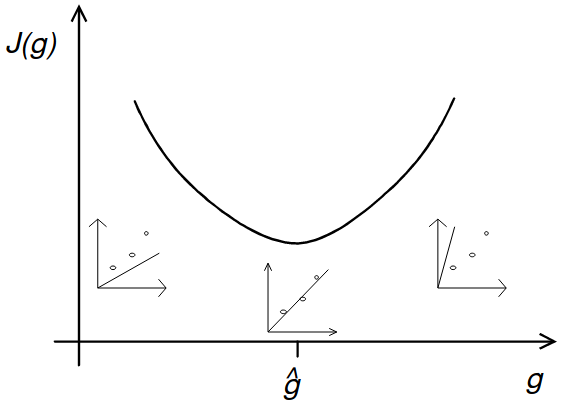
\includegraphics[width=0.5\textwidth]{img/least-aquare/Fcurve.png}
    \caption{Retas de ajuste mediante $\alpha$.}
    \label{fig:curvaF}
\end{wrapfigure}

$$
    J(\alpha) = \dfrac{1}{2}\sum_{i=1}^{n} (Y_i - \alpha X_i)^2
$$

\noindent O minimizante do funcional é obtido através da derivada em ordem ao parâmetro a estimar:
$$
    \dot{J}(\alpha) = \sum_{i=1}^{n} X_i(Y_i - \overline{\alpha} X_i) = 0
$$

\noindent A legitimidade do minimizante calculado é averiguada com recurso à segunda derivada\footnotemark[3]:
$$
    \ddot{J}(\alpha) > 0 
$$
\noindent\textbf{Nota 1}$\rightarrow$ A multiplicação de $J$ pelo escalar $1/2$ serve apenas para eliminar o termo 2 advindo da regra do expoente aquando a realização da derivada do funcional. Não influencia o cálculo do minimizante, já que estamos a igualar a derivada a 0.
\\\\
\noindent\textbf{Nota 2}$\rightarrow$ Para relações teórica que envolvam a estimação de mais do que um parâmetro, a segunda derivada deixa de ser um escalar, a legitimidade é assegurada mediante a matriz, que deve ser \underline{definida positiva}.

\footnotetext[3]{Assegura que a concavidade da curva do funcional está virada para cima, garantindo que $J(\alpha)$ seja um mínimo.}

\begin{theo}[\underline{Def.:} Matriz Definida Positiva]{}
   Se $\pmb{A}\, [n\times n]$ é uma matriz definida positiva, então os elementos da diagonal de $\pmb{A}$ são estritamente positivos, ou seja, $a_{ii} > 0, i = 1, \dots, n$. 
   
   \noindent \textbf{Nota:} Todos os valores próprios de $\pmb{A}$ são positivos ($\lambda_i > 0,\; \forall i \in \mathbb{N}$).
\end{theo}
%//==============================--@--==============================//%
\clearpage
\subsection[5.2 Notação Matricial]{$\rightarrow$ Notação Matricial}
Supondo uma equação às diferenças do género:
$$
    y(t) = a_1 y(t-1) + \dots + a_n y(t-n) = b_0 u(t-1) + \dots + b_m u(t - 1 - m)
$$
\noindent Define-se o vetor de parâmetros a estimar como:
$$
    \theta = \begin{bmatrix} a_1 & \dots & a_n & b_1 & \dots & b_n  \end{bmatrix}^\text{T}
$$
\noindent E o regressor como:
$$
    \varphi(t - 1) = \begin{bmatrix} -y(t-1) & \dots & -y(t-n) & u(t-1) & \dots & u(t-1-m)  \end{bmatrix}^\text{T}
$$
\noindent O modelo deduzido pode ser escrito como:

$$
    y(t) = \varphi(t - 1)\theta + \varepsilon(t) \rightarrow \text{Para n observações}
$$

$$
    \underbrace{\begin{bmatrix} y(1) \\ y(2) \\ \vdots \\ y(n) \end{bmatrix}}_{Y_e}= 
    \underbrace{\begin{bmatrix}  \varphi(0) \\ \varphi(1) \\ \vdots \\ \varphi(n - 1)\end{bmatrix}}_{\Phi}
    \begin{bmatrix} a_1 \\ a_2 \\ \vdots \\ a_n\end{bmatrix} + 
    \begin{bmatrix} \varepsilon(1) \\ \varepsilon(2) \\ \vdots \\ \varepsilon(n)\end{bmatrix}
$$

\noindent Onde $\varepsilon(t)$ é um resíduo que traduz a existência de erros experimentais, que se assumem (tipicamente) pequenos, deprezáveis. 
%//==============================--@--==============================//%
\subsection[5.3 Equação Normal]{$\rightarrow$ Equação Normal}
Consequentemente, a estimativa dos mínimos quadrados do vetor parâmetros $\theta$ do modelo acima descrito é por:
$$
    \Phi^{T}\Phi\bar{\theta} =  \Phi^{T}Y_e
$$

\noindent Denominada equação normal. Se $\Phi^{T}\Phi$ existir e for invertível então a estimativa dos mínimos quadrados existe e é única.
%//==============================--@--==============================//%